In this chapter, I assess the feasibility of free-breathing 2D radial PC MRI for PWV measurements in a cohort of middle-to-late age subjects. This work is an extension of prior work in which I incorporate more rigorous inclusion criteria based on data quality to provide more reliable comparisons and analyze the reliability of pulse wave velocity transit-time algorithms in vivo~\cite{robertsAdvancingFunctionalAssessment2023}. The updated simultaneous multi-slice acquisition described in Chapter~\ref{ch:phantom} was implemented after the LIFE study had completed and as such was not included in this chapter. However, it is explored in greater detail in Chapter~\ref{ch:respiration}. This work resulted in 1 first author abstract~\cite{narenComparingRobustnessRespiratoryresolved2024} and a first author manuscript currently under preparation. 

\section{Introduction}\label{sec:life_intro}
Arterial stiffness is a well-established early predictor for cardiovascular risk. In particular, increased aortic stiffness has been linked with numerous cardiovascular diseases such as stroke, hypertension, and coronary artery disease~\cite{sutton-tyrrellElevatedAorticPulse2005}. Aging is strong contributor to arterial stiffening, largely due to biochemical and structural alterations that thicken the vessel wall and reduce the aorta's ability to buffer pulsatile blood flows~\cite{vatnerVascularStiffnessAging2021,cavalcanteAorticStiffness2011}. Recent studies have indicated that increased aortic stiffness may also be linked to cranial pathologies such as vascular dementia and Alzheimer's Disease (AD)~\cite{deroosMagneticResonanceImaging2017,batemanPulseWaveEncephalopathy2004}. Many of the risk factors associated with neurodegeneration such as smoking, hypertension, and the apolipoprotein E4 (APOE4) gene are also associated with cardiovascular disease~\cite{hughesReviewPotentialRole2015,nordestgaardSharedRiskFactors2022,angoffAorticStiffnessEpidemiology2021}. As such, there is high clinical interest in accurately assessing arterial stiffness. 

Direct measurement of arterial stiffness is challenging; however, pulse wave velocity (PWV) provides a feasible alternative for assessing arterial stiffness through its relationship with arterial stiffness via the Moens-Korteweg equation (see Equation~\ref{eq:moens-korteweg})~\cite{newmanValidityMoensKortewegEquation1978, callaghanRelationshipPulsewaveVelocity1986}. Measurements of PWV rely on transit time measurements which are performed by recording flow or pressure waveforms at multiple locations along a vessel and calculating temporal shifts between them. This requires accurate flow measurements with high temporal resolutions as well as vascular path length measures (see Equation~\ref{eq:time_shift})~\cite{wentlandReviewMRIbasedMeasurements2014}. Multiple algorithms exist to calculate these time-shifts, some of which are described in Section~\ref{sec:phantom_methods}, yet there is no consensus on which method is optimal for PWV calculation. This is in part due to how different methods are more or less sensitive to different sources of noise and variability in the acquired waveforms, which can be influenced by the acquisition method and parameters~\cite{vardoulisValidationNovelExisting2013}. For example, the 4 transit time methods utilized in Section~\ref{sec:phantom_methods}---time-to-point (TTP)~\cite{groeninkBiophysicalPropertiesNormalsized2001,doguiMeasurementAorticArch2011}, time-to-foot (TTF)~\cite{lundstromPulseWaveVelocity2022}, time-to-upstroke (TTU)~\cite{doguiMeasurementAorticArch2011}, and cross-correlation (XCOR)~\cite{fieldenNewMethodDetermination2008}---each operate on different features of the waveforms (see Figure~\ref{fig:tt_algos}) and thus can result in different values of PWV despite operating on the same waveforms. 

As discussed in Chapter~\ref{ch:phantom}, Magnetic Resonance Imaging (MRI) has emerged as a promising avenue for non-invasively measuring time-shifts through 2D Phase Contrast (PC) imaging which enables quantification of blood velocity and flow through a plane~\cite{wentlandReviewMRIbasedMeasurements2014}. These can be combined with anatomical images for determining accurate vessel path lengths, which methods such as ultrasound or pressure wires are unable to provide, leading to more robust PWV calculations. Standard cine 2DPC cardiac imaging is acquired with Cartesian sequences which require breath-holds to avoid respiratory motion artifacts. However, many elderly, senile, or health-compromised patients such including those with AD, are incapable of holding their breath or following breathing directions which can result in severely compromised image quality. The radial free-breathing 2D phase contrast sequence introduced in Chapter~\ref{ch:phantom} provides a promising alternative that can enable PWV measurements in these patient populations. Additionally, the radial acquisitions, plus a longer acquisition time enabled by free-breathing, allow for retrospectively increasing the temporal resolution which can be beneficial for capturing faster transit times. 

The motivation of this chapter is to assess the feasibility of a free-breathing, radially undersampled 2DPC sequence for aortic PWV measurements by comparing to a standard, Cartesian 2DPC breath-hold sequence. Additionally, constrained reconstruction techniques are utilized to increase the temporal resolution of the acquired radial data to investigate the effects of increased temporal resolution on PWV\@. Aortic PWV measurements are obtained in a cohort of middle-aged, cognitively unimpaired adults with three 2DPC methods (Cartesian, standard radial, and high temporal resolution radial) to assess the relationship between aortic PWV and age and compare the impact of 4 different transit time algorithms on calculated PWVs.

\section{Materials \& Methods}\label{sec:life_methods}
Data for this study comes from the Longitudinal Impact of Fitness and Exercise (LIFE) study, which consists of a subset of the greater Wisconsin Alzheimer's Disease Research Center (ADRC) Clinical Core and the Wisconsin Registry for Alzheimer's Prevention (WRAP) observation cohorts. The LIFE study seeks to characterize the longitudinal relationship between cardiorespiratory fitness (CRF) --— a physiological indicator for habitual physical activity --— and the cognitive features of AD\@. Furthermore, it aims to assess vascular and glucoregulatory function as potential mechanisms underlying the beneficial effects of CRF and so PWV measures were obtained as a marker for vascular health\@. 

The subjects included in this study consist of cognitively healthy middle-aged adults as well as older individuals at elevated risk for AD, characterized in part by a higher prevalence of the APOE4 genotype and a parental history of AD\@. Eligibility criteria for the LIFE study required participants to be at least 45 years of age and free from cognitive impairment or deficits in decision-making capacity at enrollment, as determined by standardized neuropsychological assessments~\cite{jackNIAAAResearchFramework2018,langhoughkoscikValidityEvidenceResearch2021}. Exclusion criteria included current use of antipsychotic medications and general contraindications to MRI, such as pregnancy or the presence of magnetically activated implants. Written informed consent was obtained from all participants and investigations were conducted in compliance with HIPAA regulations and the University of Wisconsin-Madison Health Sciences Institutional Review Board. In total, 150 subjects were recruited for the study.

\subsubsection{MR Imaging Protocol}
As part of the longitudinal assessment, participants were imaged twice over the course of the study with a baseline exam at the start of the study and a follow-up exam two years later to assess changes in CRF and cerebrovascular health due to habitual exercise. During the course of the study, the scanner model, imaging coil, and location were changed from a 3T Discovery MR750 with an 8-channel chest coil (GE Healthcare, Waukesha, WI) located at the Waisman Center (Madison, WI) to a 3T SIGNA Premier with a 30-channel chest coil (GE Healthcare, Waukesha, WI) located at the Wisconsin Institutes of Medical Research (WIMR) (Madison, WI). To ensure data consistency, only the follow-up visit data acquired at the WIMR location collected between January 2023 and December 2024 were included in the study resulting in 83 cases (see Figure~\ref{fig:life_sort}). 

\begin{figure}[ht]
    
    \centering
    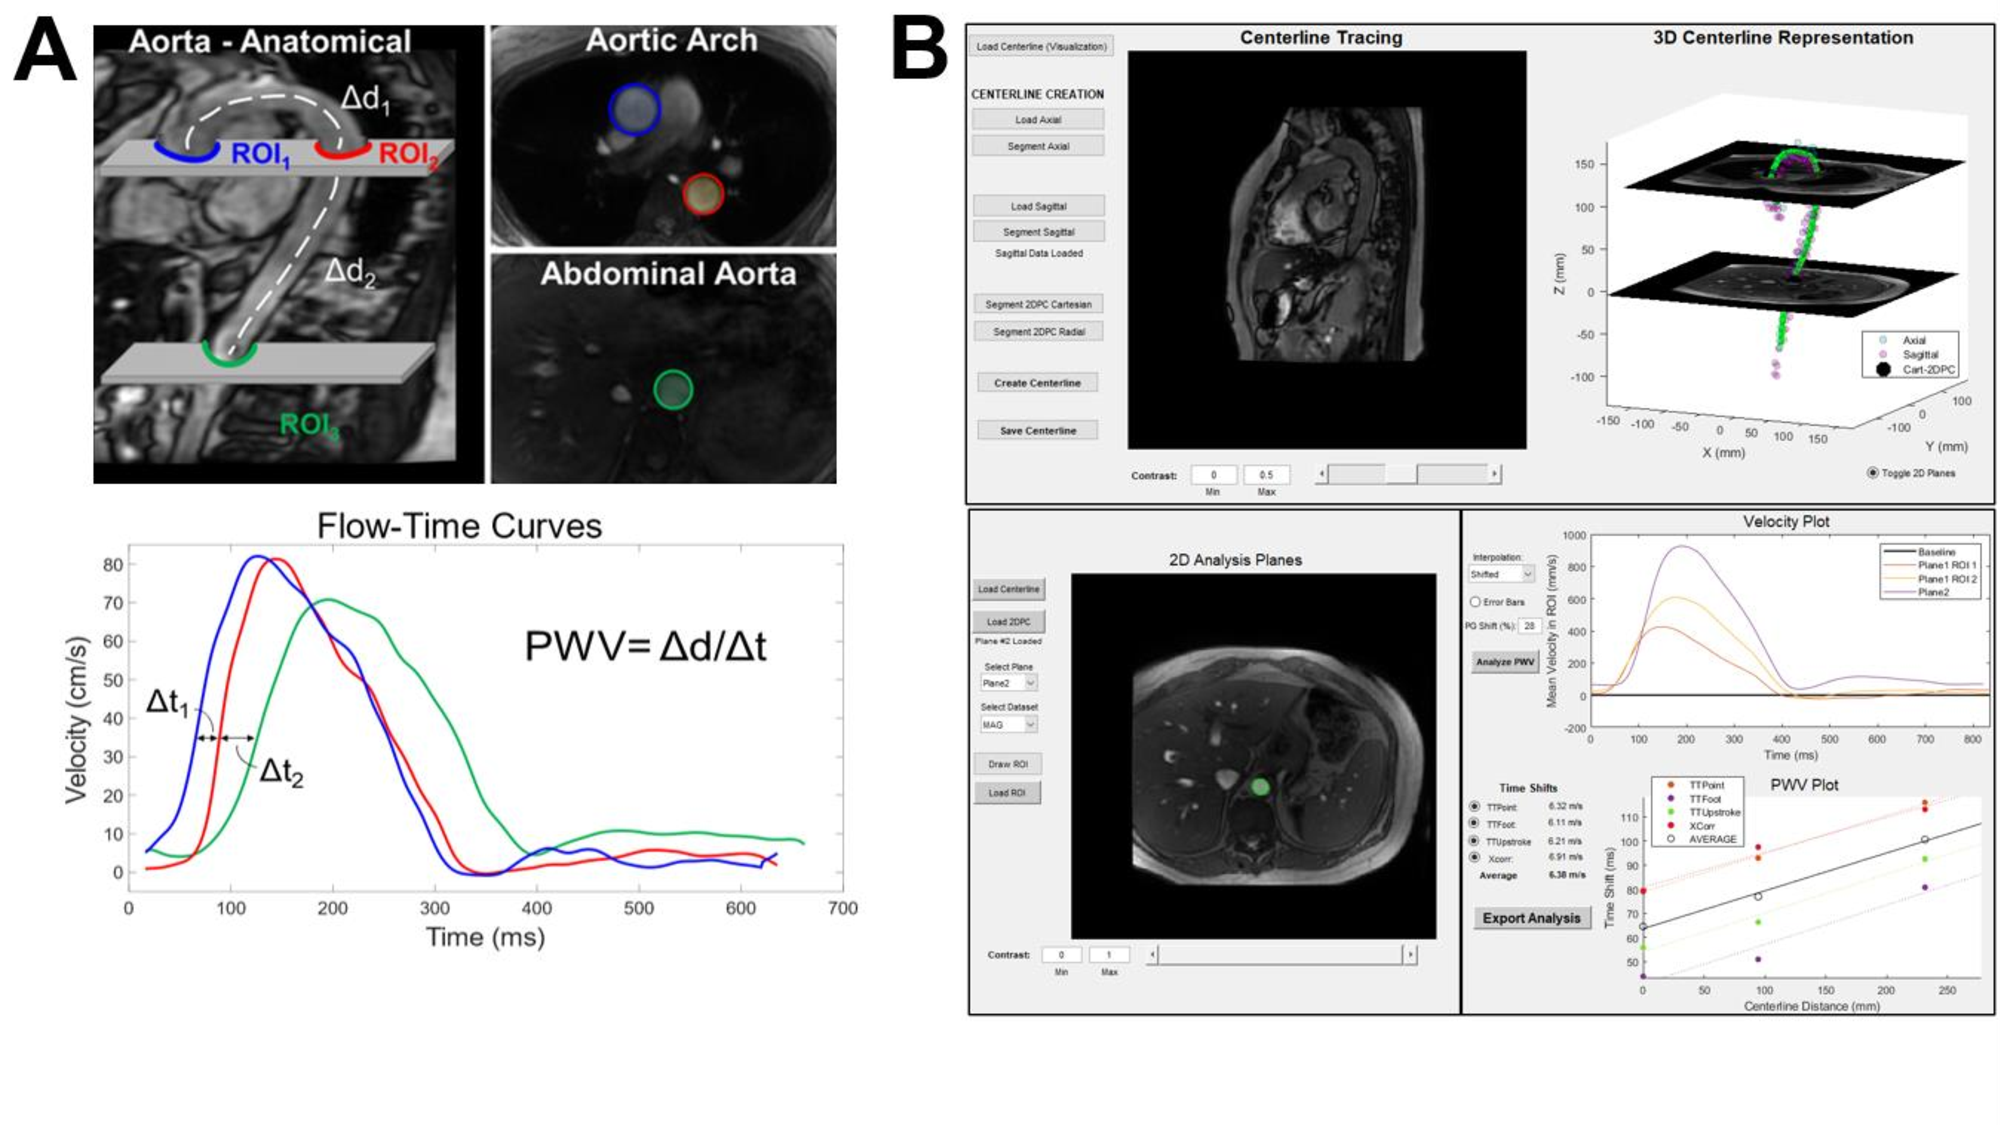
\includegraphics[page=1, width=\textwidth, alt={A Example scan prescription for the MRI acquisitions. B The MATLAB based user interface for pulse wave velocity analysis}]{PWV_figures.pdf}

    \caption[PWV analysis tool]{Overview of the 2D Phase Contrast (2DPC) acquisition and pulse wave velocity (PWV) analysis framework. (A) Two axial planes were acquired for each PC scan, one bisecting the aortic arch and the other in the abdomen, for a total of three aortic ROIs. (B) A custom software platform was developed to segment the aorta ROIs, trace aortic centerlines, analyze flow curves, and calculate PWV\@. Figure courtesy of Grant Roberts.}\label{fig:pwv_tool}
    
\end{figure}

For the chest scans, ungated anatomical balanced steady state free precession (bSSFP) product sequences (axial, coronal, sagittal) were acquired to guide aortic centerline tracing and vessel path length calculation. Parameters for the scans are identical to the ones acquired and described in Section~\ref{sec:phantom_methods}. For the Cartesian and radial 2DPC sequences, two axial planes were placed along the aorta. The superior slice was prescribed in the aortic arch at the level of the pulmonary bifurcation while the inferior slice was prescribed just above the radial arteries. This resulted in the acquisition of 3 total regions of interest (ROIs) in the aorta: the ascending and descending aortas in the superior slice and the abdominal aorta in the inferior slice (Figure~\ref{fig:pwv_tool}A). Table~\ref{tab:LIFE_scan_params} lists the scan parameters for both types of acquisitions. Photoplethysmography (PPG) data from a peripheral pulse oximeter attached to the index finger and respiratory data from respiratory bellows  attached to the chest were recorded during 2DPC acquisitions for retrospective physiological gating. 

\begin{table}[ht]
    \centering
    \caption[LIFE study scan parameters]{Acquisition parameters for 2D Cartesian and radial 2D phase contrast scans.}\label{tab:LIFE_scan_params}
    \small
    \tagpdfsetup{table/header-rows={1}}
    \vspace{0.25cm}
    \begin{tabular}{lccc}
    \toprule
    \textbf{Parameter} & \textbf{Cartesian 2DPC} & \textbf{Radial 2DPC} \\
    \midrule
    TR / TE (ms) & 5.1 / 3.1 & 7.5 / 4.3 \\
    Flip angle & 25$^\circ$ & 25$^\circ$ \\
    Views per segment & 4 & N/A \\
    Sampling & Cartesian & Golden-Angle \\
    Acquired FOV (cm) & 36 & 32 \\
    Acquired spatial resolution (\qty{}{\mm^2}) & $1.41 \times 1.41$ & $1.40 \times 1.40$ \\
    Slice thickness (mm) & 6 & 5 \\
    Venc (cm/s) & 150 & 150 \\
    Velocity encoding & 2-point & 2-point \\
    Number of projections & N/A & 10,000 \\
    Scan time & 12--20s & 150 s \\
    \bottomrule
    \end{tabular}
\end{table}

Cartesian acquisitions were automatically reconstructed on the scanner post-acquisition by the GE Healthcare product reconstruction engine. For the radial acquisition, offline reconstructions were performed with a custom reconstruction framework developed in C++. Two different types of radial reconstructions were employed: a standard reconstruction designed to match the Cartesian acquisition using Parallel Imaging with Localized Sensitivities (PILS) (standard radial) and a constrained reconstruction using a local low rank (LLR) algorithm to increase spatial and temporal resolution (hi-res radial)~\cite{griswoldPartiallyParallelImaging2000, jimenezFeasibilityHighSpatiotemporal2018,haldarLowrankApproximationsDynamic2011}. Both reconstructions utilized ESPIRiT coil sensitivity estimation for parallel imaging and included Maxwell term phase offset corrections, and gradient calibration to correct trajectory errors~\cite{ueckerESPIRiTEigenvalueApproach2014, bernsteinConcomitantGradientTerms1998, johnsonImproved3DPhase2008}. The iterative LLR reconstruction was performed with nuclear norm regularization using a local block size of 4 $\times$ 4 $\times$ 4 and an empirically determined regularization parameter of $\lambda$ = 0.003 for 55 iterations. All data were reconstructed in end-exhalation using a 50\% threshold of the respiratory waveform performed with a sliding 10-second window to account for respiratory drift. Table~\ref{tab:recon_params} lists the reconstructed parameters for all image types.

\begin{table}[ht]
    \centering
    \caption[2D phase contrast reconstructed parameters]{Reconstruction parameters for Cartesian, radial low-res, and radial hi-res 2D phase contrast scans. PILS = Parallel Imaging with Localized Sensitivities, LLR = Local Low Rank constrained reconstruction \\
    *Temporal resolutions are dependent on heart rate and are reported as mean $\pm$ standard deviation for the cohort.}\label{tab:recon_params}
    \small
    \tagpdfsetup{table/header-rows={1}}
    \vspace{0.25cm}
    \begin{tabular}{lccc}
    \toprule
    \textbf{Parameter} & \textbf{Cartesian 2DPC} & \textbf{Standard Radial} & \textbf{Hi-Res Radial} \\
    \midrule
    Reconstruction type & Vendor default & PILS & LLR \\
    Reconstructed matrix & $256 \times 256$ & $256 \times 256$ & $320 \times 320$ \\
    Reconstructed spatial resolution & $1.41 \times 1.41$ & $1.40 \times 1.40$ & $1.00 \times 1.00$ \\
    Reconstructed cardiac frames & 40 & 40 & 80 \\ 
    Temporal resolution* (ms) & 26.2 $\pm$ 3.6 & 25.2 $\pm$ 3.6 & 12.5 $\pm$ 1.8  \\ 
    \bottomrule
    \end{tabular}
\end{table}

\subsubsection{Analysis}
PWV calculations for each subject and statistical analyses were performed in MATLAB (version 2020b, Mathworks, Natick, MA) using the GUI tool described in detail in Section~\ref{sec:phantom_methods} by a single observer (T.N. with 5 years experience in 2DPC MRI analysis). Images were assessed prior to analysis for general image quality, proper plane placement, and presence of velocity aliasing. Physiological gating signals were also assessed by plotting respiratory waveforms and R-R intervals. Datasets that failed to meet quality standards for any of those reasons were excluded from analysis. The 4 time-shift methods introduced and utilized in Section~\ref{sec:phantom_methods}---TTP, TTF, TTU, and XCOR---were used to calculate PWVs for each subject with each acquisition type (Cartesian, standard radial, hi-res radial).

% Secondary analysis was performed by 3 additional observers for assessment of inter-observer variability (Figure~\ref{fig:pwv_interobserver}).

Aortic centerline distances and pulse wave velocities (PWVs) were summarized for the full cohort according to age groups (50--59, 60--69, and 70--79 years) and sex. For each variable, the mean, standard deviation, and sample size (N) were reported. Differences in PWV across acquisitions for each time-shift method were evaluated using the Friedman test. PWV distributions are visualized with box plots, showing medians, variability, and outliers, with paired measurements connected by line segments.

Associations between acquisition and time-shift method pairs were assessed using Pearson correlation coefficients ($r$) and visualized with a correlation matrix. To evaluate the relationship between age and aortic PWV, simple linear regression models were constructed for each acquisition and time-shift method. Regression coefficients ($\beta$), coefficients of determination ($R^2$), and corresponding p-values were reported, with statistical significance defined as $p < 0.05$.

\section{Results}\label{sec:life_results}
Of the 83 subjects examined in this study, 21 were excluded due to: poor plane prescription (8), insufficient image quality or velocity aliasing (11), or poor cardiac or respiratory gating (2) in one or more of the three acquisition types. An additional 17 subjects were excluded due to calculated PWVs with one or more of the implemented time-shift algorithms resulting in a physiologically impossible value (PWV $<$ 1 m/s or PWV $>$ 20 m/s). This resulted in a final total of 45 cases included in this analysis (Figure~\ref{fig:life_sort}). Demographics information for these 45 subjects are shown in Table~\ref{tab:life_demo}. 

\begin{figure}[ht]
    
    \centering
    \includegraphics[page=4, width=\textwidth, alt={Flowchart indicating the number of subjects utilized in this study and exclusion criteria}]{PWV_figures.pdf}

    \caption[LIFE subject exclusion flow chart]{The LIFE study recruited 150 subjects for 2 visits two years apart. Of the 116 subjects who returned for the follow-up visit, 33 were excluded due to being scanned at a different location and scanner system. Of the remaining 83, 11 were excluded due to poor image quality (from to various imaging artifacts), 8 due to poor scan prescription (imaging planes placed too high or low), and 2 due to poor gating quality (noisy cardiac or respiratory signals). Furthermore, an additional 17 subjects were excluded due to calculated PWVs with one or more algorithms being non-physiological (PWV $<$ 1 m/s or PWV $>$ 20 m/s). Data for the resulting 45 subjects are presented here.}\label{fig:life_sort}
    
\end{figure}

Average $\pm$ standard deviation temporal resolutions for the Cartesian, standard radial, high-res radial reconstructions were 26.2 $\pm$ 3.6 ms, 25.2 $\pm$ 3.6 ms, and 12.5 $\pm$ 1.8 ms, respectively. Plane distances (in the superior-inferior direction) between the aortic arch and abdominal aorta 2D slices were 131 $\pm$ 18.3 mm. Representative images from each of the 3 acquisition methods are shown in Figure~\ref{fig:rad_images}. Image quality in all acquisitions was sufficient for flow quantification and PWV analysis. Radial images contained some undersampling streak artifacts around the edges of the torso. Table~\ref{tab:life_pwvs} provides aortic lengths between each of the 3 measurement locations and PWV values for each acquisition and time-shift method by the whole group, age category, and by sex. Average PWV across the entire cohort ranged from 7.1--7.7 m/s for each time-shift method.

\begin{table}[ht]
    \centering
    \caption[Patient demographics]{Patient demographics for analyzed study subjects (N=45). For continuous data, values are expressed as mean $\pm$ SD and data ranges are in parentheses. For categorical data, values are expressed as numerators with percentage in parentheses. \\
    *Race was self-reported and obtained as required by federal funding agencies \\
    **APOE4 = apolipoprotein E4}\label{tab:life_demo}
    \small
    \tagpdfsetup{table/header-rows={1}}
    \vspace{0.25cm}
    \begin{tabular}{ll}
    \toprule
    \textbf{Variable} & \textbf{Value} \\
    \midrule
    Age (years) & $63.1 \pm 7.41$ (50--77) \\
    Sex & \\
    \quad Female & 34 (76\%) \\
    \quad Male & 11 (24\%) \\

    Race* & \\
    \quad White & 44 (97.8\%) \\
    \quad Unknown & 1 (2.2\%) \\

    Education (years) & $16.8 \pm 1.98$ (12--20) \\

    Parental history of dementia & \\
    \quad Yes & 36 (80.0\%) \\
    \quad No & 9 (20.0\%) \\

    Parental history of AD & \\
    \quad Yes & 23 (51.1\%) \\
    \quad No & 9 (20.0\%) \\
    \quad Unknown & 13 (28.9\%) \\

    APOE4 carrier** & \\
    \quad Yes & 30 (66.7\%) \\
    \quad No & 14 (31.1\%) \\
    \quad Unknown & 1 (2.2\%) \\
    \bottomrule
    \end{tabular}
\end{table}

Friedman test results demonstrated a significant difference in PWV across acquisition methods for the TTP algorithm ($\chi^2 = 8.62$, $p = 0$.01) and the XCOR algorithm ($\chi^2 = 7.20$, $p = 0.03$), whereas no significant differences were observed for the TTF and TTU algorithms. Box plots illustrating PWV distributions by MRI acquisition method (Figure~\ref{fig:boxplots}) indicate that Cartesian-derived PWV values frequently deviate from those obtained using radial acquisitions, particularly at higher PWV ranges.

\begin{figure}[ht]
    
    \centering
    \includegraphics[page=5, width=\textwidth, alt={Magnitude and phase images for an example subject}]{PWV_figures.pdf}

    \caption[Radial image examples]{Examples of time-averaged and time-resolved (single frame) phase contrast images in the ascending aorta (AAo) and abdominal aorta (AbdAo) across a Cartesian product scan, a standard radial reconstruction, and a high-res (Locally Low Rank) radial reconstruction for a single subject. Time-averaged Cartesian image was constructed by averaging all reconstructed time-frames from the default vendor reconstruction. All images demonstrate sufficient image quality for pulse wave velocity analysis. Radial images contain some undersampling streak artifacts around the edges of the torso.}\label{fig:rad_images}
    
\end{figure}


\begin{table}[ht]
    \centering
    \caption[Aortic distances and pulse wave velocities]{Aortic path lengths and pulse wave velocities (PWVs) stratified by age group and sex for three different 2D phase contrast image types: Cartesian, standard radial (Std. Radial), and high temporal resolution radial (HR Radial) from four different transit time algorithms (TTP = time-to-point; TTF = time-to-foot; TTU = time-to-upstroke; XCOR = cross-correlation). All values expressed as: mean $\pm$ standard deviation.}\label{tab:life_pwvs}
    \footnotesize
    \tagpdfsetup{table/header-rows={1}}
    \vspace{0.25cm}
    \begin{tabularx}{\textwidth}{lcccccc}
    \toprule
    \textbf{Parameter} & \textbf{Overall} & \textbf{50--59} & \textbf{60--69} & \textbf{70--79} & \textbf{Male} & \textbf{Female}  \\
    & (N=45) & (N=13) & (N=17) & (N=15) & (N=11) & (N=34) \\

    \midrule
    Aortic Length & 258.0 $\pm$ 23.6 & 252.1 $\pm$ 21.1 & 257.5 $\pm$ 24.6 & 263.6 $\pm$ 24.7 & 275.8 $\pm$ 18.6 & 252.2 $\pm$ 22.3 \\

    \midrule
    % \multicolumn{7}{l}{\textbf{Cartesian}} \\
    \textbf{Cartesian} & \phantom{0} & \phantom{0} & \phantom{0} & \phantom{0} & \phantom{0} & \phantom{0} \\

    TTP  & $7.2 \pm  2.3$ & $6.5 \pm  1.2$ & $6.6 \pm  2.0$ & $8.4 \pm  2.7$ & $8.1 \pm  3.4$ & $6.9 \pm  1.7$ \\
    TTF  & $7.1 \pm  2.9$ & $6.0 \pm  0.9$ & $6.3 \pm  2.4$ & $9.1 \pm  3.6$ & $7.7 \pm  3.7$ & $6.9 \pm  2.6$ \\
    TTU  & $7.3 \pm  2.8$ & $6.2 \pm  1.0$ & $6.5 \pm  2.4$ & $9.1 \pm  3.4$ & $8.1 \pm  3.8$ & $7.0 \pm  2.3$ \\
    XCOR & $7.3 \pm  1.8$ & $7.4 \pm  1.6$ & $6.8 \pm  2.2$ & $7.8 \pm  1.7$ & $7.8 \pm  2.3$ & $7.2 \pm  1.7$ \\

    \midrule
    % \multicolumn{7}{l}{\textbf{Standard Radial}} \\
    \textbf{Std. Radial} & \phantom{0} & \phantom{0} & \phantom{0} & \phantom{0} & \phantom{0} & \phantom{0} \\

    TTP  & $7.6 \pm  1.4$ & $7.0 \pm  1.0$ & $7.2 \pm  1.3$ & $8.6 \pm  1.3$ & $7.4 \pm  1.4$ & $7.7 \pm  1.4$ \\
    TTF  & $7.6 \pm  1.9$ & $6.8 \pm  1.3$ & $7.0 \pm  1.6$ & $9.0 \pm  2.1$ & $7.3 \pm  2.4$ & $7.7 \pm  1.8$ \\
    TTU  & $7.6 \pm  1.9$ & $6.7 \pm  2.1$ & $7.2 \pm  1.6$ & $8.7 \pm  1.3$ & $7.1 \pm  2.5$ & $7.7 \pm  1.6$ \\
    XCOR & $7.8 \pm  2.1$ & $7.7 \pm  1.9$ & $7.7 \pm  2.5$ & $7.9 \pm  2.0$ & $7.4 \pm  2.0$ & $7.9 \pm  2.1$ \\


    \midrule
    % \multicolumn{7}{l}{\textbf{Hi-Res Radial}} \\
    \textbf{HR Radial} & \phantom{0} & \phantom{0} & \phantom{0} & \phantom{0} & \phantom{0} & \phantom{0} \\

    TTP  & $7.5 \pm  1.3$ & $7.1 \pm  1.2$ & $7.1 \pm  1.2$ & $8.2 \pm  1.0$ & $7.3 \pm  1.4$ & $7.5 \pm  1.2$ \\
    TTF  & $7.3 \pm  1.6$ & $6.6 \pm  1.2$ & $6.9 \pm  1.5$ & $8.4 \pm  1.5$ & $7.1 \pm  2.0$ & $7.4 \pm  1.5$ \\
    TTU  & $7.3 \pm  1.7$ & $6.4 \pm  2.0$ & $7.1 \pm  1.4$ & $8.3 \pm  1.1$ & $7.2 \pm  1.7$ & $7.3 \pm  1.7$ \\
    XCOR & $7.6 \pm  2.0$ & $7.5 \pm  2.1$ & $7.4 \pm  2.1$ & $7.8 \pm  1.9$ & $7.2 \pm  2.1$ & $7.7 \pm  2.0$ \\

    \bottomrule
    \end{tabularx}
\end{table}


\begin{figure}[ht]
    
    \centering
    \includegraphics[page=6, width=\textwidth, alt={Four box plots for demonstrating pulse wave velocity distributions for each transit time method and acquisition type.}]{PWV_figures.pdf}

    \caption[PWV distributions across methods]{Distributions of pulse wave velocities calculated using four different transit time methods across a Cartesian product scan, a standard radial reconstruction, and a high-res (Locally Low Rank) radial reconstruction. Connecting lines between paired data points highlight the individual correlations on a participant level.}\label{fig:boxplots}
    
\end{figure}

Pearson correlation coefficients for each combination of time-shift method and acquisition are presented as a correlation matrix in Figure~\ref{fig:correlation}A, with all pairwise correlations reaching statistical significance. Mean correlations averaged across acquisitions (i.e., within each transit time method) are shown in Figure~\ref{fig:correlation}B. The highest mean correlations were observed for TTF (mean $r = 0.73$) and XCOR (mean $r = 0.72$) when compared across acquisitions, whereas comparisons between different transit time methods yielded lower correlations. Mean correlations averaged across transit time methods are displayed in Figure~\ref{fig:correlation}C. The Cartesian acquisition demonstrated the highest mean inter-method correlation (mean $r = 0.80$), although strong correlations were also observed for the standard radial (mean $r$ = 0.73) and high temporal resolution radial (mean $r = 0.72$) acquisitions. While transit times between the two radial acquisitions were strongly correlated (mean $r$ = 0.67), correlations between Cartesian and radial acquisitions were comparatively weak (mean $r < 0.28$). 

\begin{figure}[ht]
    
    \centering
    \includegraphics[page=7, width=\textwidth, alt={A Corelation matrix for all transit time methods and acquisition types. B Correlation averaged across acquisitions. C Correlations averaged across transit time methods}]{PWV_figures.pdf}

    \caption[PWV correlations]{(A) Correlation matrix of Pearson correlation coefficients between individual pairs of transit time methods and acquisitions. The transit time methods include Time-To-Point (TTP), Time-To-Foot (TTF), Time-To-Upstroke (TTU), and Cross-Correlation (XCOR) while the acquisitions include a Cartesian product sequence, a standard radial reconstruction, and a high temporal resolution (Locally Low Rank) radial reconstruction. (B) Mean correlations averaged across acquisitions (C) Mean correlations averaged across transit time methods}\label{fig:correlation}
    
\end{figure}

Simple linear regression analysis revealed a significant association between aortic PWV and age for the TTP, TTF, and TTU methods in both standard and high-res radial acquisitions, whereas no significant relationship was observed for the XCOR method. In contrast, the Cartesian acquisition demonstrated a significant relationship between PWV and age for the TTF and TTU methods only, with no significant associations for TTP or XCOR\@. Representative regression plots for the TTF method across all three acquisitions are provided in Figure~\ref{fig:linear_regression}. For the TTF method, regression coefficients for age ($\beta_{age}$) ranged from 0.06 to 0.11 m/s, with corresponding $R^2$ values between 0.16 and 0.22 and standard errors between 0.03 and 0.04. Among all approaches, the high temporal resolution radial acquisition exhibited the strongest relationship with age, with $R^2$ values ranging from 0.02 to 0.20 across methods.

\begin{figure}[ht]
    
    \centering
    \includegraphics[page=8, width=\textwidth, alt={Three linear regression plots comparing pulse wave velocity with age for each acquisition type.}]{PWV_figures.pdf}

    \caption[PWV linear regression with age]{Linear regression models showcasing the positive relationship between age and pulse wave velocity calculated via the Time-to-Foot method in three different acquisitions: a Cartesian product sequence, a standard radial reconstruction, and a high-res (Locally Low Rank) radial reconstruction.}\label{fig:linear_regression}
    
\end{figure}

\section{Discussion}\label{sec:life_discussion}
In this study, we implemented a radial, free-breathing two-dimensional phase contrast (2DPC) MRI sequence and assessed the feasibility of utilizing it for measuring aortic pulse wave velocity (PWV). The radial free-breathing approach was evaluated against a standard clinical breath-hold Cartesian acquisition. The radial data was used to reconstruct two different datasets: one with spatial and temporal resolution matched to the Cartesian acquisition, and a second with enhanced spatial and temporal resolution achieved with a constrained local low-rank (LLR) reconstruction. PWVs were calculated via 4 different transit time algorithms for each of the three acquisitions to compare the impact of acquisition type and transit time method on PWV estimates. The relationship between age and aortic PWV was also assessed for each acquisition and transit time method pair.

Radial data utilized in this study was heavily undersampled with approximately 250 projections per cardiac frame for the standard reconstruction. This resulted in some streaking artifacts around the edges of structures and vessels which could then manifest as noise within the derived flow waveforms. However, as PWV calculations rely on time-shifts between flow waveforms, it is likely that PWV analysis is robust to undersampling artifacts as long as the upstroke portion of the flow waveform maintains its general shape between acquisitions. The LLR reconstruction doubled the temporal resolution by halving the number of projections per frame but still resulted in comparable image quality. It was hypothesized that higher temporal resolutions would enhance the accuracy of PWV measurements, but while the high temporal resolution dataset did demonstrate the strongest correlation with age, in most other aspects, the results were largely similar to the standard radial. 

While the radial reconstructions showed strong agreement for all algorithms, there was less agreement between the Cartesian and radial reconstructions, as indicated by the difference in correlations (Figure~\ref{fig:correlation}) and paired line segments in the box plots (Figure~\ref{fig:boxplots}). There are several possible contributors to this observation, such as gating timing issues resulting from separate acquisitions, respiratory effects of breath-holds vs free-breathing, or differences in the post-processing between automatically-reconstructed Cartesian images and the radial reconstructions. Additionally, heart rate variability between the two acquisitions may also be a contributing factor as breath-holds have been shown to have effects on heart rate~\cite{hassanEffectNormalBreathing2021a}.

All acquisitions and transit time methods (aside from XCOR) showed significant relationships with age. Specifically, we found that aortic PWV increases by around 1.1--1.4 m/s each decade of life. This agrees closely with a large study (N=397) performed by van Hout et al., in which they assessed aortic PWV in older adults (mean age 55 $\pm$ 6 years) using 2DPC MRI~\cite{vanhoutNormalReferenceValues2021}. They observed an average PWV increase of 0.9 m/s over 10 years. Similar results have been demonstrated in other 2DPC MRI studies~\cite{dyverfeldtPulseWaveVelocity2014,parikhMeasurementPulseWave2016, hicksonRelationshipAgeRegional2010}. Furthermore, the study by van Hout et al.\ reported a mean PWV value of 6.8 m/s for the age range 60--65 years using the TTF method, which is similar to the results obtained here (mean PWV\textsubscript{TTF} = 6.3 $\pm$ 2.4 m/s)~\cite{vanhoutNormalReferenceValues2021}. Another study by Hickson et al.\ also reported a mean PWV in a similar age bracket of approximately 6 m/s using the TTP method which again agrees with our results (mean PWV\textsubscript{TTP} = 6.6 $\pm$ 2.4 m/s)~\cite{hicksonRelationshipAgeRegional2010}. However, a large normative study (N=777) by Nethononda et al.\ reported a mean aortic PWV of 9.6 $\pm$ 4.1 m/s in the 60--69 year age range using the TTF method which is considerably higher than what our and the other referenced studies reported~\cite{nethonondaGenderSpecificPatterns2015}. One possible explanation for this could be the number of slices acquired for PWV calculations. While our study and Nethononda et al.\ acquired 2 slices in the aorta (3 total ROIs), van Hout et al.\ acquired 3 slices (4 ROIs) and Hickson et al.\ acquired 4 slices (5 ROIs). It has been shown that the sampling density along the aorta for 2DPC based measurements can affect the accuracy of PWV calculations which may indicate that Hickson et al.\ is the most reliable value for comparison~\cite{kronerEvaluationSamplingDensity2012}.

In prior work performed on this cohort analyzing PWV, there were considerable methodological complications that compromised the reliability of the PWV analysis~\cite{robertsAdvancingFunctionalAssessment2023}. For one, data acquired for this study were tagged onto a larger cranial study and performed at a location specializing in head and neck imaging. This resulted in a number of concessions including the use of a smaller chest coil (8-channel), cardiac gating performed with PPG instead of ECG signals, and an acquisition order in which free-breathing acquisitions were performed directly after breath-hold acquisitions without time for subjects to return to a resting state. To amend these issues, during follow-up visits, scheduling was gradually adjusted to transition subjects to another location better equipped for cardiac imaging, with MR technologists more experienced in cardiac imaging and a larger chest coil (30 channel) was available. Cardiac gating was still performed with PPG signals to remain consistent with prior data, however, the acquisition order was modified to perform all breath-hold acquisitions at the beginning of the session (Cartesian scans) followed by the free-breathing acquisitions (radial scans) with the intention of reducing the variability in heart rates between acquisitions. All data analyzed in this study were acquired after these adjustments were made, with the result that while we increased our confidence in the quality of analyzed data, we experience a considerable reduction in sample size (N=117 vs N=45) and thus statistical power~\cite{robertsAdvancingFunctionalAssessment2023}. However, the updated results presented here demonstrated an overall reduction in calculated PWVs across most categories and transit time algorithms. The previous analysis reported mean PWVs across the entire cohort ranging from 7.7--8.4 m/s and for comparisons to other studies, PWV\textsubscript{TTP} and PWV\textsubscript{TTF} of 7.9 $\pm$ 3.4 and 7.8 $\pm$ 3.7, respectively~\cite{robertsAdvancingFunctionalAssessment2023}. As stated previously, our results show closer agreement with these other studies, which may indicate that the methodological adjustments we made were successful in improving the reliability of our PWV measurements.

Despite the efforts made to improve the acquisitions, a considerable number of datasets still had to be excluded in analysis due to poor prescription, image quality, or gating (21 out of 83). One potential reason for plane placement issues could be due to the unconventional prescription needed for the radial acquisition. The sequence was implemented via modification of an existing 3D radial research sequence and as such, the prescription was still performed as a 3D acquisition, requiring some effort to correctly center the volume at the desired location for the 2D slice. Additionally, as the radial images had to be reconstructed offline, immediate feedback after acquisition was not available like it was for the automatically reconstructed product Cartesian sequence, so there was no possibility of a quick re-acquisition to correct issues. On the other hand, the majority of image quality issues were present in the Cartesian images (8 of 11) due to ghosting artifacts from respiratory motion or aliasing from parallel imaging that interfered with velocity measurements. Meanwhile, a few radial images (3) demonstrated artifacts similar to the ones shown in Figure~\ref{fig:phantom_images} which may indicate issues with the sequence. Further investigation into the source of this artifact is needed. Only 2 datasets were excluded due to poor gating, which is a considerable decrease from the 17 excluded in the original analysis~\cite{robertsAdvancingFunctionalAssessment2023}. Finally, an additional 17 datasets were excluded due to physiologically impossible PWV values, an issue that was present in the original analysis as well but was accounted for by simply excluding individual values. The primary cause of these physiological impossible PWVs was likely due to changes in heart rates between acquisitions, resulting in changes to the abdominal aorta waveforms with a different period (R-R interval) and temporal resolution compared to waveforms measured in the aortic arch. When time-shifts are calculated between the waveforms, if the waveforms are too close together, it can result in very large PWVs (PWV $>$ 20 m/s), or if the waveforms overlap, it can result in negative PWVs. It should be noted also that different time-shift methods fail in different ways and that some methods may be more robust than others in different failure scenarios. For example, the TTP algorithm determines time shifts from only a single point and is thus more sensitive to outliers, but by the same token may be the least affected by heart rate variation. Meanwhile, the TTF method relies on the slopes of the waveforms and may produce negative time-shifts if later waveforms have flatter waveforms. The TTU method is dependent on identifying the point at the beginning of the upstroke through fitting of a sigmoid function but can be compromised by increased noise in the late diastolic/early systolic portion of the flow waveform which is common in 2DPC acquisitions due to the reduction in signal from reduced inflow. Lastly, the XCOR algorithm calculates time-shifts by perform correlations across the entire waveform and is thus more prone to errors from wave reflections that are present in diastole. Considering the variability in all these methods, it may be beneficial to acquire all time-shift results (which take relatively little time to compute) to provide backup measures in the event one of the algorithms fails. Wentland et al.\ also suggest that averaging multiple time-shift results together may provide the most robust PWV values~\cite{wentlandReviewMRIbasedMeasurements2014}.

\subsubsection{Limitations}
There were several limitations to this study. As discussed, changes in heart rate between acquisitions led to physiologically impossible PWV values in a number of subjects. This was present in both Cartesian and radial acquisitions and is limitation of sequential acquisitions. A 3D or interleaved acquisition that captures multiple slices simultaneously would alleviate this issue, but typically requires reduced temporal resolution or prolonged acquisition times. The simultaneous multi-slice (SMS) acquisition described in Chapter~\ref{ch:phantom} is therefore a promising alternative as it acquires multiple slices at the same time without sacrificing either of those.

Another limitation is the usage of PPG gating over more typical ECG gating for cardiac MRI\@. While ECG signals are more susceptible to noise due to magneto-hydrodynamic effects from the scanner, PPG signals could potentially have less accurate triggering due to a broader R wave peak and physiological delays from measuring the cardiac signal at the finger, which could have considerable impacts on estimated PWVs~\cite{spicherInitialEvaluationProspective2016}. Further exploration in a study acquiring both ECG and PPG signals and comparing PWVs values calculated between them may be instructive.

Lastly, one factor that was not explored in this study was the physiological effects of respiratory phase (e.g., forced breath-hold compared to free-breathing state) in PWV\@. Other studies have investigated this and noted significant differences~\cite{sobolEffectShortTermBreath2019, vainerRadialArteryPulse2023, murphyEFFECTRESPIRATIONPULSE2010}, however no exploration of the effects of free-breathing and respiratory phase has been done. With a free-breathing acquisition, it would be possible to retrospectively bin data according to respiratory phase and evaluate these effects on PWV\@. This avenue will be further explored in Chapter~\ref{ch:respiration}.

Future technical improvements could include the application of machine learning for automating aorta centerline tracing and 2DPC segmentation to decrease processing time, increase accuracy of vessel area measurements, and increase repeatability. This would also allow for an additional measure of local PWV (“QA” method), that requires accurate flow and area quantification~\cite{vulliemozEstimationLocalAortic2002}. 

\section{Conclusion}\label{sec:life_conclusion}
In conclusion, the radial, free-breathing 2DPC MRI sequence offers a viable imaging technique for assessing aortic stiffness which may be particularly beneficial for subjects with breath-hold difficulty. The radial sequence offers a great deal of flexibility for physiological gating and for image reconstruction, which allowed us to generate a high temporal resolution dataset using local low rank reconstruction. Mean pulse wave velocities were comparable between the radial and Cartesian acquisitions and are consistent with other studies, however, the correlation between paired measures is relatively poor. Pulse wave velocities were tabulated in our cohort of 45 cognitively unimpaired older adults and showed strong associations with age. Future studies should seek to study intracranial hemodynamics alongside the obtained aortic pulse wave velocity data.

\subsubsection{Acknowledgements}
Work reported in this publication was supported in part by the National Institutes of Health under award numbers: R01AG062167, RF1AG027161, P30AG062715, UL1TR002373. Special thanks to Grant Roberts for his work on this project including development of the first version of the PWV analysis tool and analysis of the baseline visit data and to Kevin Johnson for his contributions to the sequence development. Thank you also to Ozioma Okonkwo, Bri Breidenbach, Steve Kecskemeti, Laura Eisenmenger, Sarah Lose, Alyssa Pandos for facilitating this study. Thank you also to Mackenzie Jarchow, Avery Rhodes, and Anna Gaul for assisting with centerline tracing and vessel segmentation.